\documentclass[11pt]{article}

% ---- packages ----
\usepackage[margin=1in]{geometry}
\usepackage{amsmath,amssymb,amsthm}
\usepackage{graphicx}
\usepackage{booktabs}
\usepackage{multirow}
\usepackage{xcolor}
\usepackage[numbers,sort&compress]{natbib}
\usepackage{caption}
\usepackage{subcaption}
\usepackage[section]{placeins} % keep floats within the section that defines them
\usepackage[colorlinks=true,linkcolor=blue!55!black,citecolor=blue!55!black,urlcolor=blue!55!black]{hyperref}

% Float placement: allow more/larger floats per page and keep them near text.
\renewcommand{\topfraction}{0.92}
\renewcommand{\bottomfraction}{0.75}
\renewcommand{\textfraction}{0.07}
\renewcommand{\floatpagefraction}{0.75}
\setcounter{topnumber}{3}
\setcounter{totalnumber}{5}

\graphicspath{{figures/}}
\newtheorem{proposition}{Proposition}
\newcommand{\kl}{\mathrm{KL}}
\newcommand{\ppl}{\mathrm{ppl}}
\newcommand{\E}{\mathbb{E}}
\newcommand{\R}{\mathbb{R}}
\newcommand{\W}{\mathbf{W}}
\newcommand{\x}{\mathbf{x}}
\DeclareMathOperator{\tr}{tr}
\DeclareMathOperator*{\argmin}{arg\,min}

\title{\textbf{TurboPress}: A Measurement-Driven Study of Rotated Low-Bit\\
Weight Quantization --- Equilibration Exponents, Error Feedback,\\
and Per-Layer Bit Allocation}

\author{Godson Johnson\\ \texttt{godsonj64@gmail.com}}
\date{Preprint.}

\begin{document}
\maketitle

\begin{abstract}
We present \textbf{TurboPress}, an instrumented post-training quantization (PTQ)
pipeline for large language model (LLM) weights, together with a set of
controlled A/B measurements that isolate the contribution of each design choice
at \emph{exactly matched} bit budgets. Building on the incoherence-processing
line of work \citep{chee2023quip,tseng2024quipsharp,tseng2024qtip,ashkboos2024quarot}
and on the rotation+optimal-quantizer construction of TurboQuant
\citep{zandieh2025turboquant}, TurboPress combines a seeded randomized
orthogonal rotation, trellis-coded quantization (TCQ) with data-free
trellis-optimized codebooks, GPTQ/LDLQ error feedback
\citep{frantar2023gptq,chee2023quip}, and per-layer bit allocation. Our
contributions are primarily \emph{empirical and analytical} rather than a claim
of a new state of the art: (i) a corrected rotation-aware \emph{equilibration
exponent}---we show that in the weight-only, post-rotation regime the optimal
per-channel fold is a quarter power $s_j=(\E[x_j^2]/\lVert \W_{:,j}\rVert^2)^{1/4}$,
distinct from the square-root heuristic of AWQ/SmoothQuant
\citep{lin2024awq,xiao2023smoothquant} and from the weight--activation balancing
result of BASE-Q \citep{he2025baseq}; (ii) a rigorous \emph{negative result} that
unbiased (QJL-style) residual correction, while provably debiasing, loses to a
finer deterministic quantizer at equal budget for weights; and (iii) an
end-to-end measurement on Qwen3-0.6B showing that error feedback and trellis
coding are complementary (trellis wins at 2 bits; both are near-lossless at 4
bits), and that KL-sensitivity-driven mixed precision beats uniform precision at
an equal $3.0$-bit budget. All numbers are reported with a KL divergence
``visible-loss'' metric and exact storage accounting; code and configuration are
released.
\end{abstract}

\section{Introduction}
Low-bit weight quantization is the dominant lever for shrinking LLM memory and
bandwidth. The strongest modern PTQ methods share a common backbone:
\emph{incoherence processing} (a random or learned rotation) to spread outliers
\citep{chee2023quip,ashkboos2024quarot,liu2024spinquant}, an
information-theoretically strong quantizer (vector or trellis codebooks)
\citep{tseng2024quipsharp,tseng2024qtip,vanderouderaa2024pvq}, and Hessian-aware
\emph{error feedback} \citep{frantar2022obc,frantar2023gptq}. TurboQuant
\citep{zandieh2025turboquant} adds a Quantized Johnson--Lindenstrauss (QJL)
sketch \citep{zandieh2024qjl} to make inner-product estimates \emph{unbiased}.

This paper does not propose a new frontier method. Instead we ask a narrower,
measurable question: \emph{at matched bit budgets, how much does each component
actually buy, and why?} We build TurboPress as a harness in which rotation,
quantizer, equilibration, error feedback, and bit allocation can each be toggled
and measured against a full-precision reference using KL divergence
$\kl(p_{\text{fp}}\Vert p_q)$, top-1 next-token agreement, and perplexity, with
storage reported to the exact fractional bit.

\paragraph{Contributions.}
\begin{itemize}\itemsep2pt
  \item \textbf{Corrected equilibration exponent (\S\ref{sec:equil}).} Under a
  rotation-based quantizer whose error is isotropic in the rotated basis, the
  expected output error factorizes as
  $\left(\sum_j c_j s_j^2\right)\!\left(\sum_j m_j/s_j^2\right)$ with
  $c_j=\lVert\W_{:,j}\rVert^2$ and $m_j=\E[x_j^2]$; Cauchy--Schwarz gives the
  optimum $s_j=(m_j/c_j)^{1/4}$. This is a \emph{quarter} power, not the square
  root used by AWQ/SmoothQuant, and it arises from a different objective than
  the weight--activation balance that yields the $1/2$ power in BASE-Q.
  \item \textbf{Error feedback in rotated coordinates (\S\ref{sec:ldlq}).} We
  implement GPTQ/LDLQ in the rotated, equilibrated basis via a fast transform of
  the activation Hessian, and show on Qwen3-0.6B that it reduces $2$-bit KL by
  $5.0\times$ and $3$-bit KL by $5.3\times$ over nearest rounding, at $\sim\!3\times$
  lower quantization cost than TCQ.
  \item \textbf{Per-layer bit allocation (\S\ref{sec:alloc}).} A measured
  KL-sensitivity probe plus a greedy budget knapsack beats uniform precision at
  an \emph{equal} $3.0$-bit budget ($\kl$ $0.238$ vs.\ $0.276$).
  \item \textbf{A refuted hypothesis (\S\ref{sec:qjl}).} Unbiased QJL residual
  correction for weights is measured to lose to deterministic quantization at
  equal budget, in both synthetic depth-compounding chains and on a real model;
  the correction's variance exceeds the bias it removes.
\end{itemize}

\section{Background and Related Work}
\paragraph{Rotation / incoherence processing.} QuIP \citep{chee2023quip} showed
that pre- and post-multiplying weights by random orthogonal matrices makes them
incoherent, tightening rounding guarantees; QuIP\# \citep{tseng2024quipsharp},
QuaRot \citep{ashkboos2024quarot}, and SpinQuant \citep{liu2024spinquant} refine
this with Hadamard and learned rotations. A random rotation renders the rotated
coordinates approximately Gaussian, which is the regime where the Lloyd--Max
scalar quantizer \citep{lloyd1982,max1960} is optimal.

\paragraph{Quantizers.} Beyond scalar rounding, vector and trellis codebooks
close much of the gap to the rate--distortion bound. Trellis-coded quantization
(TCQ) \citep{marcellin1990tcq}, built on Ungerboeck set partitioning
\citep{ungerboeck1982}, was recently applied to LLM weights by QTIP
\citep{tseng2024qtip}; Pyramid Vector Quantization is another route
\citep{vanderouderaa2024pvq}.

\paragraph{Error feedback.} OBQ/GPTQ \citep{frantar2022obc,frantar2023gptq}
quantize input channels sequentially and propagate rounding error through the
inverse Hessian; LDLQ \citep{chee2023quip} is the equivalent within incoherence
processing. Qronos \citep{zhang2025qronos} generalizes the correction step.

\paragraph{Activation-aware scaling / equilibration.} Weight equalization
\citep{nagel2019dfq}, SmoothQuant \citep{xiao2023smoothquant}, and AWQ
\citep{lin2024awq} rescale channels by (a power of) their activation magnitude;
AWQ grid-searches the exponent $\alpha\in[0.25,0.75]$. BASE-Q \citep{he2025baseq}
derives an optimal scale via AM--GM for the \emph{weight-and-activation} setting,
obtaining a square-root form. Recent concurrent work combines several of these
ingredients: QAM-W \citep{sharma2026qamw} pairs Hadamard rotation with a
grid-tuned AWQ scale and a 2D codebook; OrbitQuant \citep{lee2026orbitquant}
uses a rotated basis with a Lloyd--Max codebook and no per-channel scaling; PiSO
\citep{amboage2026piso} computes exact per-channel scales algorithmically. We
position our equilibration result precisely against these in \S\ref{sec:equil}
and \S\ref{sec:discussion}.

\section{Method}
Let a linear layer compute $\mathbf y=\W\x$ with $\W\in\R^{m\times d}$. TurboPress
replaces $\W$ by a quantized $\hat\W$ acting on a transformed input, exactly
factoring the computation as
\begin{equation}
\mathbf y=\W\x=\big(\W\,\mathbf D\,\mathbf R^\top\big)\big(\mathbf R\,\mathbf D^{-1}\x\big),
\qquad \mathbf z:=\mathbf R\,\mathbf D^{-1}\x,
\label{eq:factor}
\end{equation}
where $\mathbf D=\mathrm{diag}(\mathbf s)$ is an activation-aware equilibration and
$\mathbf R$ is a seeded randomized orthogonal transform (block Walsh--Hadamard
$\times$ Rademacher signs, with an exact dense fallback for odd dimensions). We
quantize $\W''=\W\mathbf D\mathbf R^\top$ and run
$\mathbf y\approx\hat\W''\mathbf z+\mathbf b$. All of $\mathbf R$, $\mathbf D$, and the
codebook are seeded and reproducible; only the low-bit codes and per-row scales
are stored.

\subsection{Rotation-aware equilibration: the quarter-power rule}
\label{sec:equil}
The rotation spreads the per-row quantization error approximately isotropically
across the $d$ rotated coordinates. We model the error $\mathbf E''=\W''-\hat\W''$
in the equilibrated basis as column-decorrelated with per-entry second moment
proportional to the row energy: $\E[(\W'\!-\hat\W')_{ij}^2]\approx\delta_i^2$ with
$\delta_i^2=(\varepsilon^2/d)\lVert\W''_{i,:}\rVert^2=(\varepsilon^2/d)\sum_j s_j^2 W_{ij}^2$,
where $\varepsilon^2$ is the normalized quantizer MSE and $\W'=\W\mathbf D$.

\begin{proposition}[Optimal equilibration under isotropic rotated error]
\label{prop:quarter}
With $c_j=\lVert\W_{:,j}\rVert^2$ and $m_j=\E[x_j^2]$, the expected squared
output error satisfies
\begin{equation}
\E\lVert\Delta\mathbf y\rVert^2\;\approx\;\frac{\varepsilon^2}{d}
\Big(\textstyle\sum_j c_j s_j^2\Big)\Big(\textstyle\sum_j m_j/s_j^2\Big),
\label{eq:factorized}
\end{equation}
which, by the Cauchy--Schwarz inequality, is minimized when $c_j s_j^2\propto m_j/s_j^2$,
i.e.
\begin{equation}
\boxed{\,s_j=\big(m_j/c_j\big)^{1/4}\,=\,\big(\sqrt{\E[x_j^2]}\,/\,\lVert\W_{:,j}\rVert\big)^{1/2}.}
\label{eq:quarter}
\end{equation}
\end{proposition}

\begin{proof}[Sketch]
The output error in row $i$ is
$\Delta y_i=\sum_j(\W'\!-\hat\W')_{ij}\,x_j/s_j$. Column decorrelation of the
rotated error kills cross terms in expectation, giving
$\E[\Delta y_i^2]\approx\delta_i^2\sum_j m_j/s_j^2$. Summing over $i$ and using
$\sum_i\delta_i^2=(\varepsilon^2/d)\sum_j s_j^2\sum_i W_{ij}^2=(\varepsilon^2/d)\sum_j c_j s_j^2$
yields \eqref{eq:factorized}. Cauchy--Schwarz on the two sums gives equality
when the summands are proportional, which is \eqref{eq:quarter}.
\end{proof}

\paragraph{Interpretation.} The AWQ/SmoothQuant fold $s_j\propto\E[x_j^2]^{1/2}$
is optimal only when the quantizer error stays \emph{column-aligned} (its
variance in column $j$ scales as $s_j^2 W_{ij}^2$). The random rotation destroys
that alignment---the error becomes isotropic across rotated coordinates---so the
two competing terms in \eqref{eq:factorized} both scale with the weight column,
and the optimum shifts to a quarter power. This is a distinct regime from
BASE-Q \citep{he2025baseq}, whose $1/2$ exponent balances \emph{activation}
quantization noise against \emph{weight} quantization noise (both quantized);
here activations are not quantized. The prediction $\alpha\approx 1/4$ is
consistent with the empirically favored small AWQ exponents ($\alpha\in[0.25,0.75]$,
\citealp{lin2024awq}) and the frozen $\alpha{=}0.3$ of QAM-W
\citep{sharma2026qamw}. We treat this as a narrow analytical result under stated
modeling assumptions, not a claim of a new method (\S\ref{sec:discussion}).

\subsection{Data-free trellis-optimized codebooks}
We use rate-$R$ TCQ with a doubled ($2^{R+1}$-level) codebook and a rate-1/2
convolutional trellis over $S$ states; Viterbi decoding selects the
minimum-distortion codeword \emph{sequence} per row, storing exactly $R$
bits/weight (1 path bit + $R{-}1$ member bits, verified by an
encode$\to$decode round-trip test). Because the rotation makes the coordinate
distribution known ($\approx\!\mathcal N(0,1)$), we re-optimize the codebook
\emph{under the trellis} with generalized Lloyd iterations on synthetic
Gaussians---no calibration data---and cache the result.

\subsection{GPTQ/LDLQ error feedback in rotated coordinates}
\label{sec:ldlq}
Nearest rounding leaves each layer's output error as a fixed bias. LDLQ/GPTQ
\citep{chee2023quip,frantar2023gptq} instead quantize input channels
sequentially and feed each channel's rounding error forward into the
not-yet-quantized channels, weighted by the layer's input Hessian
$\mathbf H=\E[\x\x^\top]$, minimizing
$\tr[(\W''-\hat\W'')\,\mathbf H_z\,(\W''-\hat\W'')^\top]$ rather than raw weight MSE.
The relevant Hessian in the transformed space of \eqref{eq:factor} is
$\mathbf H_z=\mathbf R\,\mathbf D^{-1}\mathbf H\,\mathbf D^{-1}\mathbf R^\top$, which we form
with two applications of the fast transform ($O(d^2\log d)$). The random rotation
is exactly the incoherence preprocessing that makes LDLQ effective. Storage and
bit accounting are identical to the plain scalar path; only the chosen codeword
changes. When $\mathbf H_z$ is diagonal, LDLQ provably reduces to independent
nearest rounding (a unit test verifies bit-exact equivalence).

\subsection{Per-layer bit allocation by measured KL sensitivity}
\label{sec:alloc}
Layers differ in sensitivity, so a uniform width wastes budget. For each
quantized linear and each candidate width $b\in\{2,3,4\}$ we quantize
\emph{only} that layer (others full precision) and measure
$\kl(p_{\text{fp}}\Vert p_q)$ on a held-out probe set---a direct, model-faithful
sensitivity signal. We then choose a width per layer to minimize total predicted
KL subject to a parameter-weighted average-bit budget, solved greedily by
repeatedly spending the next unit of budget on the upgrade with the largest KL
drop per added bit. Greedy is exact here because per-layer KL is empirically
convex-decreasing in bits.

\subsection{A refuted hypothesis: unbiased (QJL) correction for weights}
\label{sec:qjl}
TurboQuant's QJL sketch \citep{zandieh2024qjl,zandieh2025turboquant} makes a
layer output an \emph{unbiased} estimate of the full-precision output. The
hypothesis we test: since deterministic rounding produces a fixed per-layer
bias that could compound through depth, spending bits on an unbiasing sketch
might beat spending them on a finer deterministic quantizer. We implement the
1-bit QJL residual sketch (with the exact unbiasedness and variance bound
$\mathrm{Var}[\hat{\langle r,x\rangle}]\le(\pi/2)\lVert r\rVert^2\lVert x\rVert^2/k$)
and measure it at equal budget.

\section{Experimental Setup}
We quantize every $\texttt{nn.Linear}$ in the decoder blocks of a Hugging Face
causal LM (embeddings, LM head, and norms kept in full precision) and compare to
the unquantized model on real text (a fixed public-domain corpus). Primary model:
Qwen3-0.6B \citep{qwen3_2025} (28 blocks, 196 linears) in fp16 on a single
8\,GB GPU; scale-up reference: SmolLM2-135M \citep{allal2025smollm2}. Metrics on
$4{,}080$ next-token positions: mean $\kl(p_{\text{fp}}\Vert p_q)$, top-1
agreement, and perplexity; equilibration scales and Hessians are calibrated on a
disjoint $2{,}048$-token slice. Bits/weight is the exact storage-weighted average
including per-row scales and codebooks. Everything is seeded and deterministic on
a given device.

\section{Results}
\subsection{Rate--distortion on Qwen3-0.6B}
Table~\ref{tab:qwen} and Fig.~\ref{fig:rd} give the full sweep (fp16 perplexity
$29.11$). Nearest rounding collapses at 2 bits (perplexity $5.6\times10^5$);
both trellis coding and error feedback rescue it, and at 4 bits both are within
$\sim\!5\%$ perplexity of full precision with $\kl\le0.10$.

\begin{table}[htbp]
\centering
\caption{Qwen3-0.6B, all 196 decoder linears quantized; fp16 perplexity $29.11$.
``+eq'' is the quarter-power equilibration of \eqref{eq:quarter}. Best per bit in
\textbf{bold}. Quantization wall-clock on one 8\,GB GPU.}
\label{tab:qwen}
\small
\begin{tabular}{lrrrrr}
\toprule
Configuration & bits/w & $\kl(p_{\text{fp}}\Vert p_q)$ & top-1 & perplexity & time (s)\\
\midrule
Nearest (rotated scalar) 2b   & 2.012 & 10.282 & 0.020 & 564{,}874 & 4.6\\
Nearest 3b                    & 3.013 & 1.641  & 0.381 & 138.66 & 4.4\\
Nearest 4b                    & 4.013 & 0.399  & 0.670 & 43.91 & 4.0\\
\midrule
TCQ($S{=}64$)+eq 2b           & 2.023 & \textbf{1.215} & \textbf{0.450} & \textbf{91.42} & 245.9\\
TCQ($S{=}64$)+eq 3b           & 3.023 & \textbf{0.289} & \textbf{0.710} & 38.58 & 245.2\\
TCQ($S{=}64$)+eq 4b           & 4.023 & \textbf{0.079} & 0.843 & 30.63 & 247.8\\
\midrule
GPTQ/LDLQ+eq 2b               & 2.023 & 2.072 & 0.383 & 177.10 & 79.0\\
GPTQ/LDLQ+eq 3b               & 3.023 & 0.312 & 0.707 & \textbf{36.28} & 88.8\\
GPTQ/LDLQ+eq 4b               & 4.023 & 0.095 & \textbf{0.844} & \textbf{30.45} & 77.2\\
\bottomrule
\end{tabular}
\end{table}

\begin{figure}[htbp]
\centering
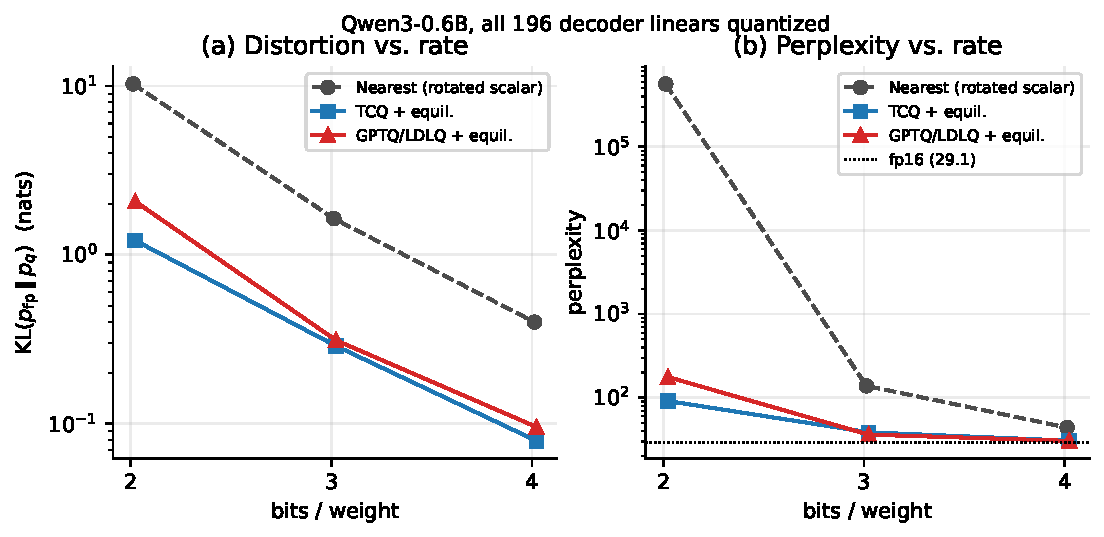
\includegraphics[width=\textwidth]{fig1_rate_distortion.pdf}
\caption{Rate--distortion on Qwen3-0.6B. Both trellis coding and error feedback
dominate nearest rounding across the whole range; they are near-lossless at
4 bits.}
\label{fig:rd}
\end{figure}

\subsection{Error feedback vs.\ trellis coding: complementary}
Fig.~\ref{fig:bars} isolates the KL of each family. Error feedback cuts 2-bit KL
$10.28\!\to\!2.07$ ($5.0\times$) and 3-bit KL $1.64\!\to\!0.31$ ($5.3\times$)
over nearest, at $\sim\!3\times$ lower cost than TCQ ($79$\,s vs.\ $246$\,s).
GPTQ/LDLQ 3b beats \emph{nearest 4b} ($\kl$ $0.312$ vs.\ $0.399$)---a full bit
saved. The two strong methods tie at 3--4 bits, but the joint trellis code wins
clearly at the hardest 2-bit setting ($\kl$ $1.22$ vs.\ $2.07$), where scalar
codebook granularity is coarsest---motivating combining them (\S\ref{sec:discussion}).

\begin{figure}[htbp]
\centering
\begin{subfigure}{0.48\textwidth}\centering
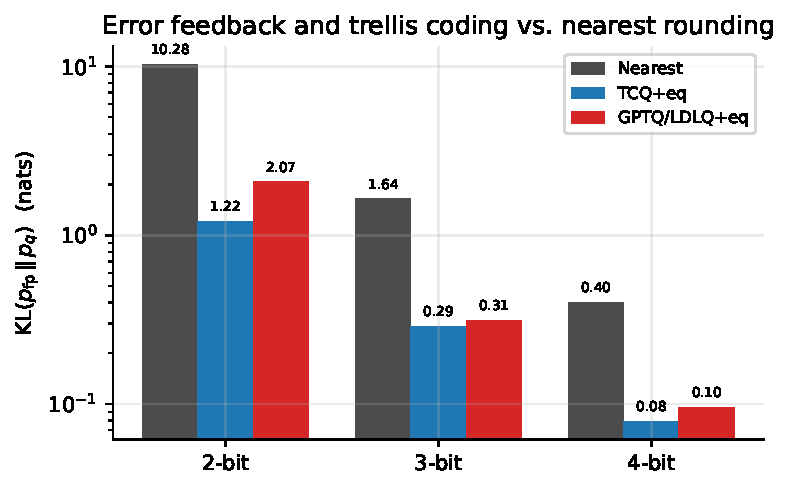
\includegraphics[width=\textwidth]{fig2_method_bars.pdf}
\caption{}\label{fig:bars}
\end{subfigure}\hfill
\begin{subfigure}{0.5\textwidth}\centering
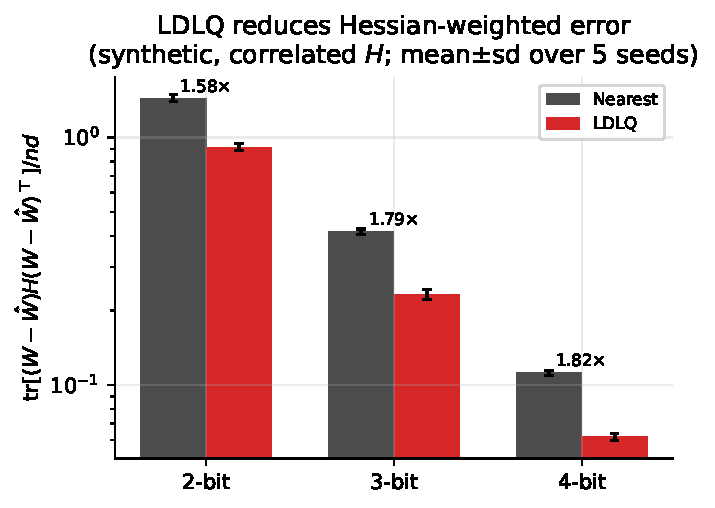
\includegraphics[width=\textwidth]{fig7_ldlq_micro.pdf}
\caption{}\label{fig:micro}
\end{subfigure}
\caption{(a) KL by method and bit-width on Qwen3-0.6B (log scale).
(b) Controlled microbenchmark: LDLQ reduces the Hessian-weighted output error
$\tr[(\W-\hat\W)\mathbf H(\W-\hat\W)^\top]/nd$ by $1.6$--$1.8\times$ over nearest on
a synthetic layer with correlated $\mathbf H$.}
\end{figure}

\subsection{The equilibration exponent matters: quarter power beats square root}
Fig.~\ref{fig:equil} tests Proposition~\ref{prop:quarter} directly: an identical
rotated scalar quantizer in which \emph{only} the activation fold changes. On
Qwen3-0.6B the quarter-power fold cuts 2-bit KL from $10.28$ (no equilibration)
to $2.40$, where the square-root fold reaches only $8.41$. On Qwen3-1.7B the
square-root fold is \emph{worse than no equilibration at all} at 3 and 4 bits
(KL $3.58$ vs.\ $2.24$, and $1.85$ vs.\ $0.64$), while the quarter fold improves
every setting ($0.46$, $0.18$). This is the failure mode \eqref{eq:quarter}
predicts: over-scaling by $\sqrt{m_j}$ inflates the folded weight energy
$\sum_j c_j s_j^2$ faster than it suppresses the activation term, and the
imbalance grows with the channel spread of the model.

\begin{figure}[htbp]
\centering
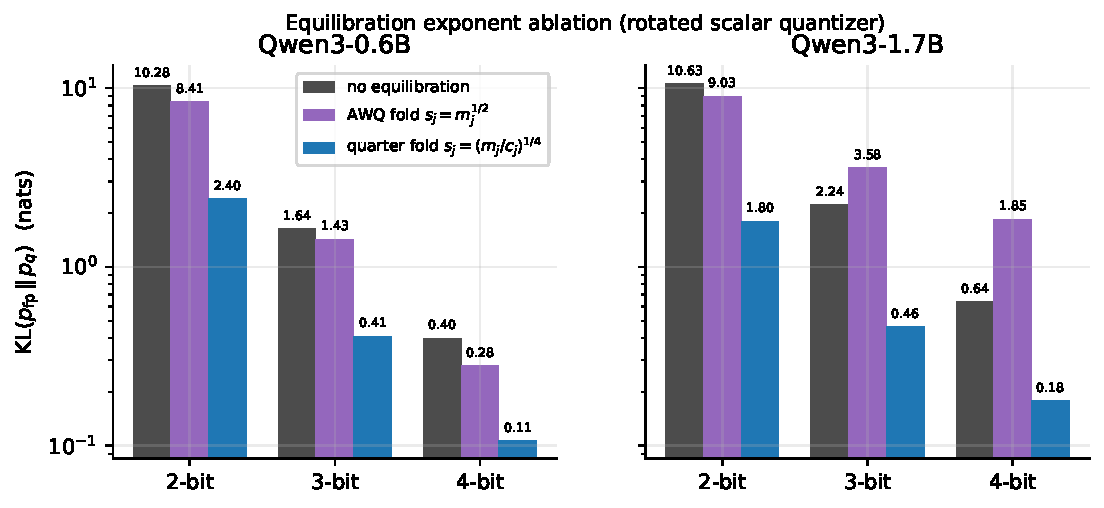
\includegraphics[width=\textwidth]{fig8_equil_exponent.pdf}
\caption{Equilibration-exponent ablation (Proposition~\ref{prop:quarter}):
identical rotated scalar quantizer, only the per-channel fold differs. The
quarter-power fold $s_j=(m_j/c_j)^{1/4}$ dominates at every bit-width on both
models; on Qwen3-1.7B the AWQ-style square-root fold is worse than no
equilibration at 3--4 bits. Log scale; calibration and evaluation slices are
disjoint.}
\label{fig:equil}
\end{figure}

\subsection{Scale-up sharpens the low-bit picture}
Fig.~\ref{fig:scale} compares SmolLM2-135M to Qwen3-0.6B for the same TCQ+eq
method. The 2-bit perplexity ratio $\ppl_q/\ppl_{\text{fp}}$ drops from $8.3\times$
($116.1/14.06$) to $3.1\times$ ($91.4/29.11$); the 4-bit perplexity gap shrinks
from $+8.1\%$ to $+5.2\%$, while 4-bit KL is essentially size-invariant
($0.0787$ vs.\ $0.0790$). Larger models quantize better at the aggressive
settings, consistent with the broader literature.

\begin{figure}[htbp]
\centering
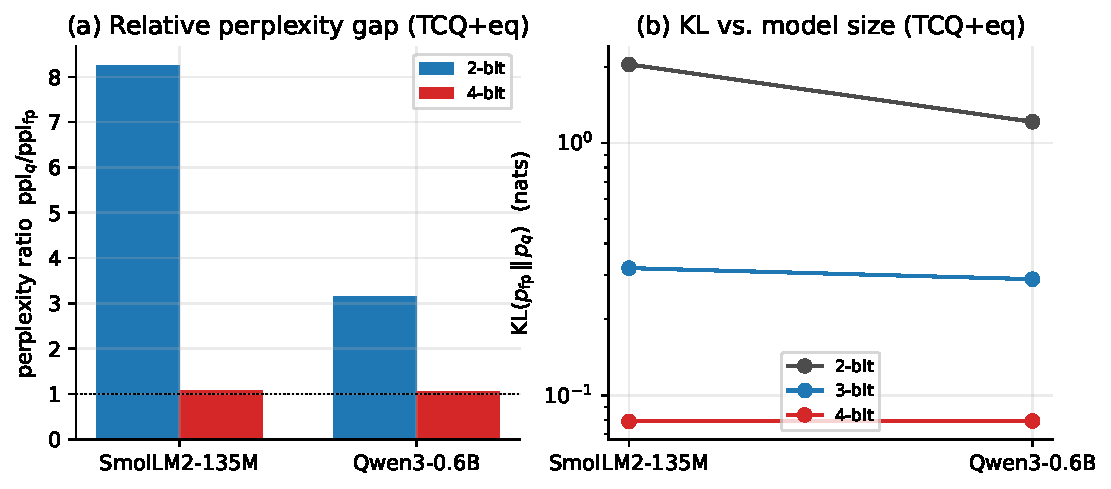
\includegraphics[width=\textwidth]{fig3_scaleup.pdf}
\caption{Scale-up from 135M to 0.6B parameters (TCQ+eq). (a) Relative perplexity
gap; (b) KL by width. The 2-bit setting improves most with scale.}
\label{fig:scale}
\end{figure}

\subsection{Per-layer bit allocation}
The sensitivity map (Fig.~\ref{fig:map}) shows MLP projections dominate
(mean single-layer 2-bit KL: down $0.0088$, up $0.0080$, gate $0.0062$), then
attention output/value ($0.0047$), with query/key nearly free ($0.0025$/$0.0016$);
block~0 and the final block are hotspots. Allocating against this signal
(Table~\ref{tab:alloc}, Fig.~\ref{fig:alloc}) beats uniform precision at an
\emph{equal} $3.0$-bit budget---$\kl$ $0.238$ vs.\ $0.276$ ($-14\%$), perplexity
$34.76$ vs.\ $36.59$---by moving 24 insensitive layers to 2 bits and 23 sensitive
ones to 4 bits. At a fractional $2.5$-bit budget (impossible for a uniform
integer width) the mixed model reaches $\kl$ $0.494$, roughly one third of the
way from uniform-2b ($1.386$) to uniform-3b.

\begin{figure}[htbp]
\centering
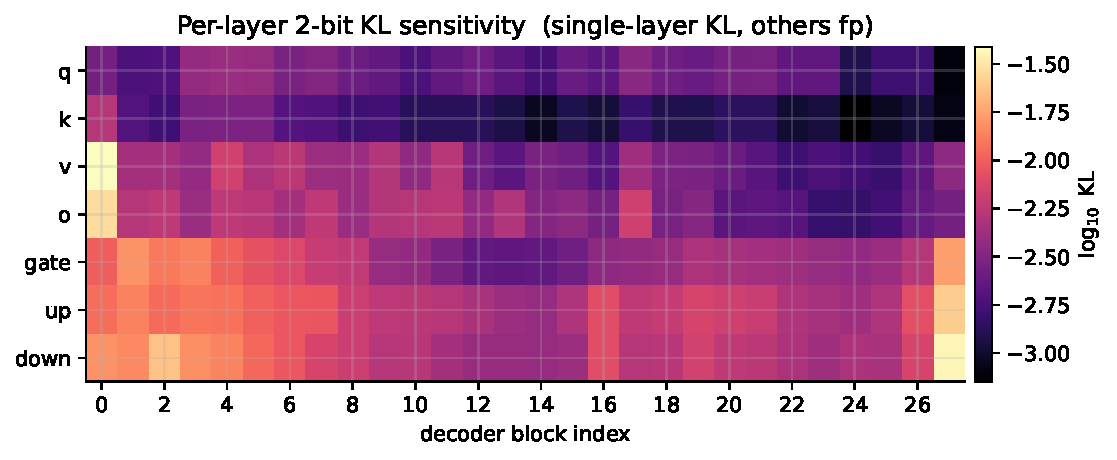
\includegraphics[width=\textwidth]{fig4_sensitivity_map.pdf}
\caption{Per-layer 2-bit KL sensitivity map (single-layer KL, others full
precision), $\log_{10}$ scale. MLP and value/output projections carry the
sensitivity; query/key are nearly free.}
\label{fig:map}
\end{figure}

\begin{table}[htbp]
\centering
\caption{Per-layer allocation vs.\ uniform (TCQ+eq, Qwen3-0.6B). The $3.0$-bit
row is an equal-budget comparison.}
\label{tab:alloc}
\small
\begin{tabular}{llrrrl}
\toprule
Budget & Model & bits/w & $\kl$ & perplexity & layers (2/3/4 bit)\\
\midrule
\multirow{2}{*}{$3.0$ (equal)} & \textbf{Mixed (allocated)} & 3.023 & \textbf{0.238} & \textbf{34.76} & 24 / 149 / 23\\
                               & Uniform 3-bit             & 3.023 & 0.276 & 36.59 & 0 / 196 / 0\\
\midrule
$2.5$ & Mixed (allocated) & 2.523 & 0.494 & 44.79 & 101 / 91 / 4\\
--    & Uniform 2-bit     & 2.023 & 1.386 & 105.18 & 196 / 0 / 0\\
\bottomrule
\end{tabular}
\end{table}

\begin{figure}[htbp]
\centering
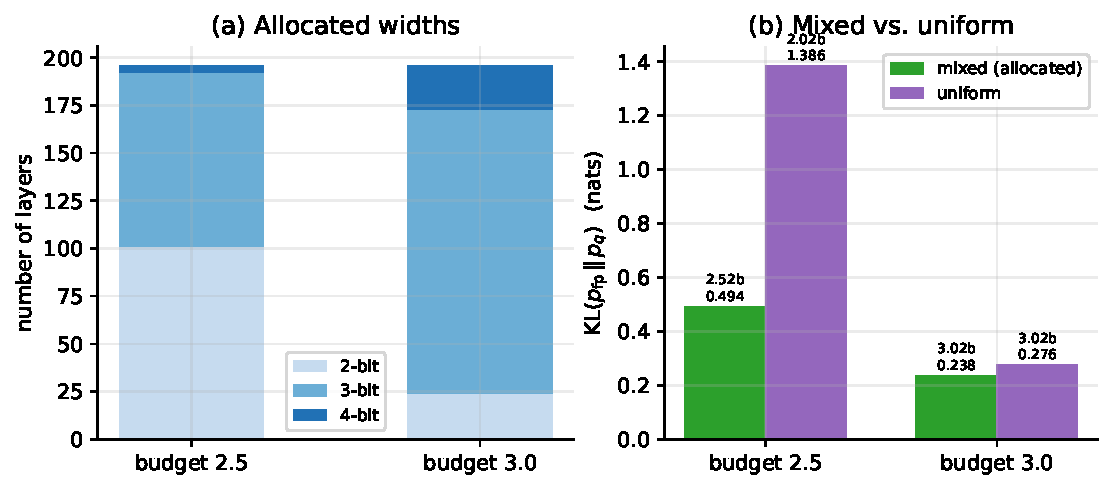
\includegraphics[width=\textwidth]{fig5_allocation.pdf}
\caption{(a) Widths chosen by the allocator at each budget. (b) KL of mixed vs.\
uniform; annotations give bits/weight and KL. At equal $3.0$ bits the mixed model
wins.}
\label{fig:alloc}
\end{figure}

\subsection{The QJL-for-weights negative result}
At an equal $\sim\!3$-bit budget, the unbiased QJL correction is markedly worse
than plain nearest 3-bit. In a 16-layer synthetic chain (Fig.~\ref{fig:qjl}),
nearest-3b reaches $\kl$ $0.096$ / top-1 $0.98$ while 2b+QJL($k{=}d$, $3.06$
bits) reaches $\kl$ $2.58$ / top-1 $0.01$; on a real 135M model at equal budget
the QJL-corrected model ($\kl$ $9.75$) is $\sim\!5.7\times$ worse than nearest-3b
($\kl$ $1.72$). The estimator debiases exactly as predicted, but its noise
standard deviation $\sqrt{\pi/2}\,\lVert r\rVert\lVert x\rVert/\sqrt{k}$ exceeds the
bias it removes even at $k{=}d$ (a full extra bit), and the variance compounds
multiplicatively through depth. The random rotation already decorrelates
residuals from activation structure, removing the failure mode the correction
targets. QJL remains the right tool where TurboQuant proved it---KV-cache /
attention inner products, where the error path is shallow.

\begin{figure}[htbp]
\centering
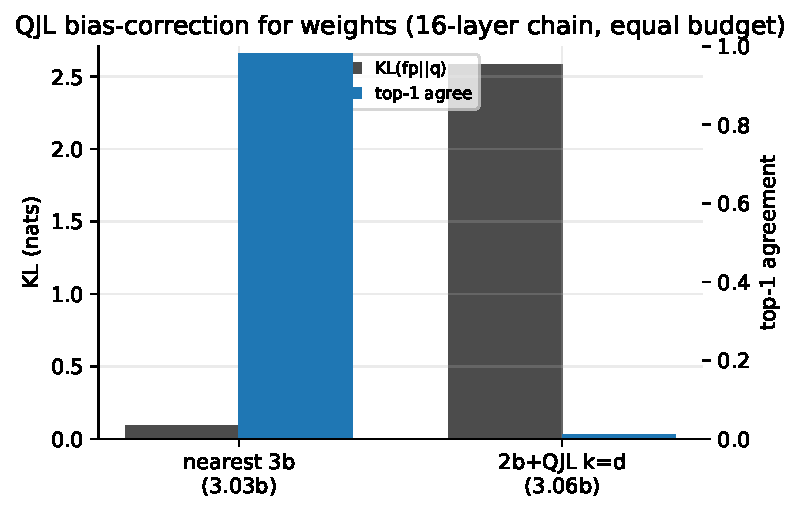
\includegraphics[width=0.55\textwidth]{fig6_qjl_negative.pdf}
\caption{Unbiased QJL correction for \emph{weights} loses to deterministic
rounding at equal budget (16-layer chain). Correction variance $>$ removed bias.}
\label{fig:qjl}
\end{figure}

\section{Discussion, Positioning, and Limitations}
\label{sec:discussion}
\paragraph{What is and is not novel.} The pipeline shape---rotation, strong
codebook, error feedback, mixed precision---overlaps substantially with recent
work \citep{tseng2024qtip,tseng2024quipsharp,he2025baseq,sharma2026qamw,lee2026orbitquant,zhang2025qronos};
we make no state-of-the-art claim. Our defensible analytical contributions are
the quarter-power equilibration exponent (Proposition~\ref{prop:quarter}), which
we position explicitly against BASE-Q's $1/2$ (a different objective) and AWQ's
grid-tuned heuristic, and the QJL-for-weights negative result. The AM--GM /
Cauchy--Schwarz \emph{machinery} for optimal scaling is itself established
\citep{he2025baseq,amboage2026piso}; only the exponent for the weight-only,
post-rotation regime is, to our knowledge, unstated elsewhere.
\paragraph{Limitations.} (i) Scale: our evidence is at $\le0.6$B parameters; the
2-bit ranking in particular may shift at 7B+. (ii) Baselines: we compare against
our own controlled configurations, not against released GPTQ/AWQ/QuIP\#/QTIP
checkpoints on WikiText-2 and zero-shot suites; those comparisons are required
before any efficiency claim. (iii) The equilibration result rests on the
isotropic-error and MSE-proportional-to-energy modeling assumptions of
\S\ref{sec:equil}; it is an approximation, not an exact optimality theorem.
(iv) Ours is a measurement implementation: dequantized weights are materialized
in the model dtype rather than packed low-bit kernels, so numerics---but not
latency---match a deployed kernel.
\paragraph{Next step.} The data point directly at combining error feedback with
the trellis (block-LDLQ over TCQ, in the spirit of QuIP\#/QTIP), since trellis
wins at 2 bits and error feedback is cheap and complementary; evaluated at 7B
against standard baselines, that combination is the natural methods contribution.

\section{Conclusion}
TurboPress is a reproducible harness that measures, at matched bit budgets, the
marginal value of each ingredient of modern rotated PTQ. Its measurements yield
a corrected equilibration exponent, a clean negative result on unbiased weight
correction, a demonstration that error feedback and trellis coding are
complementary, and an equal-budget win for KL-driven mixed precision. We release
the code, configurations, and exact result logs.

\paragraph{Reproducibility.} All experiments are seeded and deterministic on a
given device; the release includes the quantization modules, the sweep and
allocation drivers, $89$ unit tests (exact identities, statistical bounds,
trellis round-trip, LDLQ equivalence, allocation properties), and the raw result
JSON from which every table and figure is generated.

\bibliographystyle{plainnat}
\bibliography{references}

\end{document}
